\documentclass[11pt, a4paper]{article}

\usepackage{graphicx}
\usepackage[a4paper,top=3cm,bottom=2cm,left=2cm,right=2cm,marginparwidth=1.75cm]{geometry}
\usepackage[english]{babel}
\usepackage[utf8x]{inputenc}
\usepackage{subfig}
\usepackage{float}
\usepackage{amsmath}
\usepackage{amssymb}
\usepackage{mhchem}
\usepackage{hyperref}
\usepackage{tikz}
\usepackage{cancel}
\usepackage{bm}

\graphicspath{ {./images} }
\newcommand*{\qed}{\hfill\ensuremath{\quad\square}}%
\newcommand*{\rad}{\ensuremath{\,\text{rad}}}
\newcommand*{\R}{\ensuremath{\mathbb{R}}}
\newcommand*{\C}{\ensuremath{\mathbb{C}}}
\renewcommand*{\Re}{\operatorname{Re}}
\renewcommand*{\Im}{\operatorname{Im}}
\renewcommand*{\epsilon}{\varepsilon}
\renewcommand*{\phi}{\varphi}
\renewcommand*{\d}{\text{d}}

\DeclareRobustCommand{\uvec}[1]{{%
  \ifcat\relax\noexpand#1%
    % it should be a Greek letter
    \bm{\hat{#1}}%
  \else
    \ifcsname uvec#1\endcsname
      \csname uvec#1\endcsname
    \else
      \bm{\hat{\mathbf{#1}}}%
     \fi
   \fi
}}

\makeatletter
\renewcommand*\env@matrix[1][*\c@MaxMatrixCols c]{%
  \hskip -\arraycolsep
  \let\@ifnextchar\new@ifnextchar
  \array{#1}}
\makeatother

\newtheorem{theorem}{Theorem}
\numberwithin{equation}{section}
\numberwithin{figure}{section}

%------------------------------------------------
%Templates for images and figures
% \begin{figure}[h]
%   \centering
%   \subfloat[caption 1]{{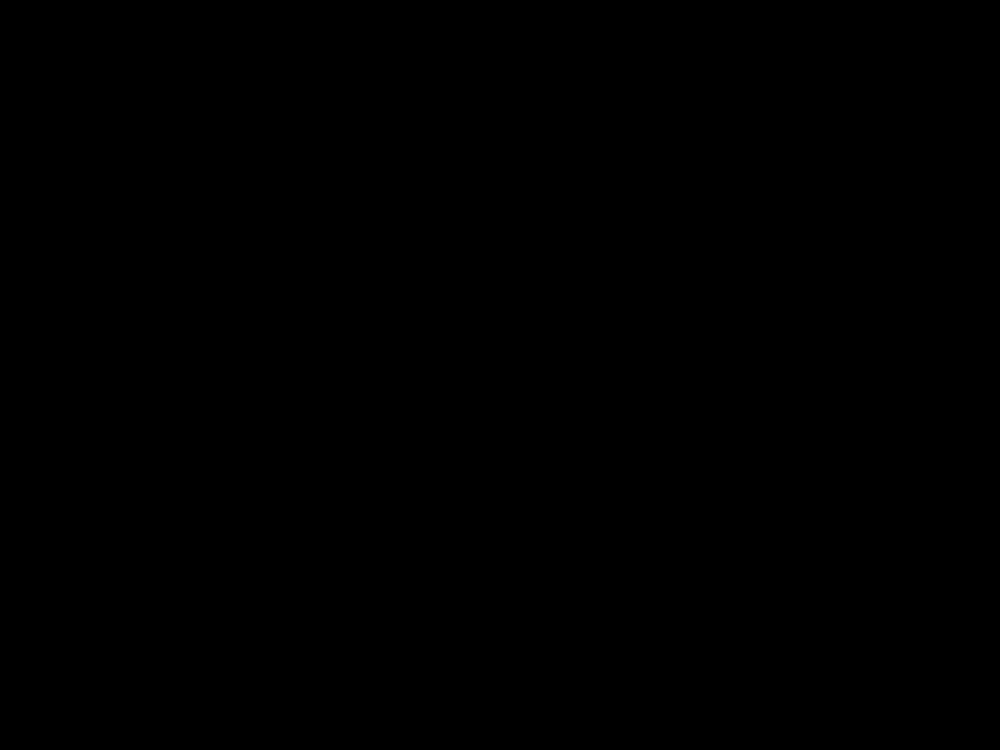
\includegraphics[width=30mm]{images/placeholder.png}}}%
%   \qquad
%   \subfloat[caption 2]{{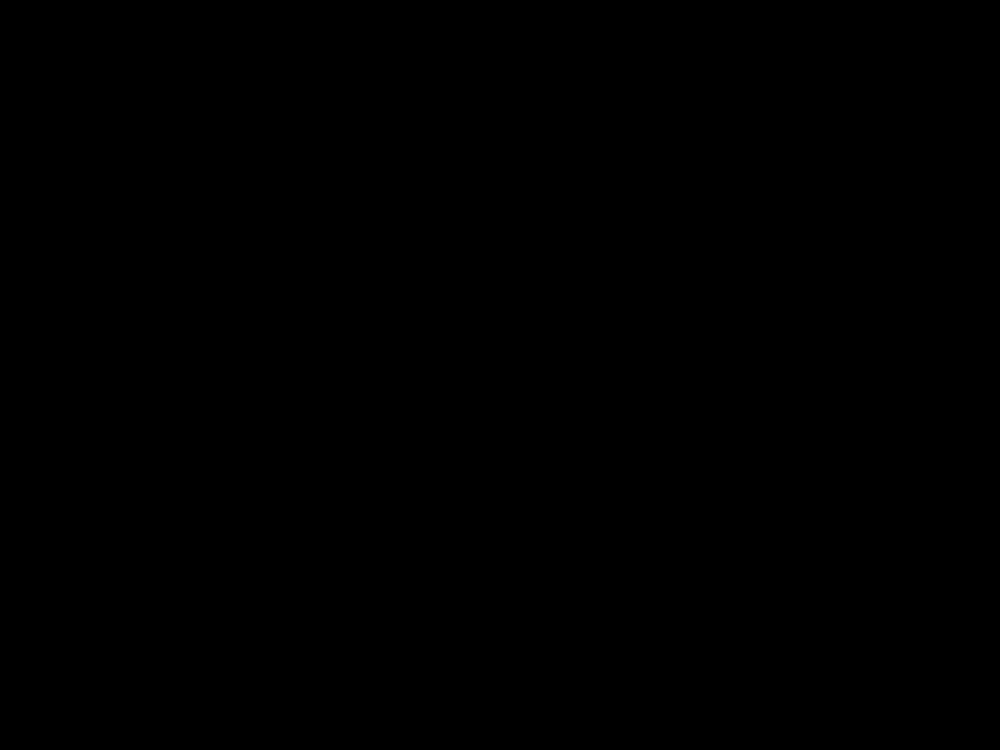
\includegraphics[width=30mm]{images/placeholder.png}}}%
%   \caption{Description}
% \end{figure}

% \begin{figure}[h]
%   \centerline{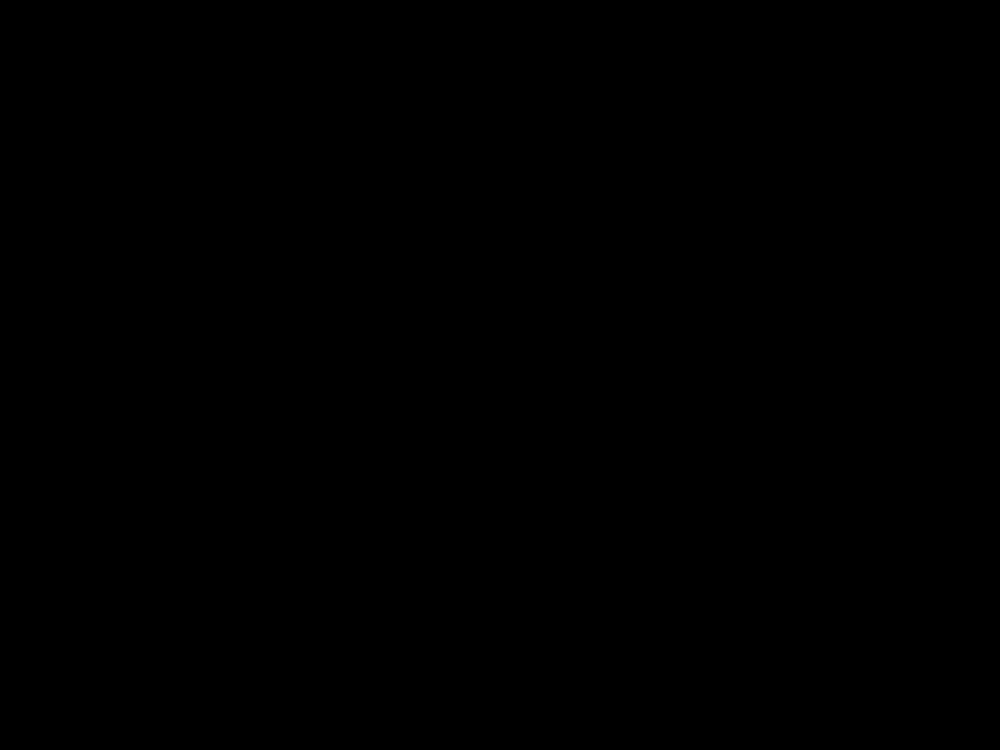
\includegraphics[width=50mm]{images/placeholder.png}}
%   \caption{Description}
% \end{figure}

%Template for a simple table 
%\begin{table}[h]
%   \caption{Description} %title of the table
%   \centering % centering table
%   \begin{tabular}{l rr} % creating three columns
%     \hline\hline %inserting double-line
%     & & \\ [0.5ex] % Insert half line vertical spacing
%     \hline % inserts single-line
%     & & \\ 
%     & & \\
%     & & \\
%     & & \\
%   \hline % inserts single-line
%   \end{tabular}
%   \label{tab:hresult}
% \end{table}
%-----------------------------------------------

\begin{document}
\setcounter{section}{1}

\subsection{The Green-Lagrange strain tensor}
Recall the relations established in lecture 1:
\begin{equation}
  \vec{r}\,' = \vec{r} + \vec{u}
\end{equation}
Where $\vec{r}\,'$ is the new position vector to the point on the deformed body, $\vec{r}$ the point on the undeformed body and $\vec{u}$ a vector which represents the displacement vector. Note that $\vec{u}$ is usually a function of $x, y$ and $z$. 
\begin{equation}
  \vec{u} = \vec{u}(x, y, z)
\end{equation}
If the original vector $\vec{r}$ is given as $\vec{r} = \langle x, y, z \rangle$, then the components of the deformed vector become:
\begin{align}
  r\,'_x &= x + u_x \notag\\
  r\,'_y &= y + u_y \notag\\
  r\,'_z &= z + u_z
\end{align}
If we take the differential of the vectors $\vec{r}\,'$ and $\vec{r}$, square them and take the differnce we get:
\begin{equation}
  \d \vec{r}\,' \cdot \d \vec{r}\,' -  \d \vec{r}\cdot  \d \vec{r} = 2
  \begin{bmatrix}
    \d x &
    \d y &
    \d z
  \end{bmatrix}
  \begin{bmatrix}
    \epsilon_{xx} & \epsilon_{xy} & \epsilon_{xz} \\
    \epsilon_{yx} & \epsilon_{yy} & \epsilon_{yz} \\
    \epsilon_{zx} & \epsilon_{zy} & \epsilon_{zz} \\
  \end{bmatrix}
  \begin{bmatrix}
    \d x \\
    \d y \\
    \d z
  \end{bmatrix}
\end{equation}
Where $\epsilon_{ij}$ is the Green-Lagrange strain tensor. The entries $\epsilon_{ij}$ can be computed using the following expression:
\begin{align}
  \epsilon_{ij} &= \frac{1}{2} \left( \frac{\partial u_i}{\partial x_j} + \frac{\partial u_j}{\partial x_i} + \sum_k \frac{\partial u_k}{\partial x_i}\frac{\partial u_k}{\partial x_j} \right)\ \notag\\
  &= \frac{1}{2}(u_{i,j} + u_{j,i} + \sum_ku_{k,i}u_{k,j})
\end{align}
For a 3 dimensional body expressed in cartesian coordinates $i,j,k=1=x$, $i,j,k=2=y$ and $i,j,k=3=z$. Recall  Clairaut's theorem (also referred to as symmetry of second derrivatives or equality of mixed partials) which states the following:
\begin{equation}
  \frac{\partial}{\partial y} \left(\frac{\partial f}{\partial x}\right) = \frac{\partial}{\partial x} \left(\frac{\partial f}{\partial y}\right)
\end{equation}
From this we can conclude that $\epsilon_{xy} = \epsilon_{yx}$. Because of this relation the Green-Lagrange tensor is a symmetric tensor. THis gives it 6 independent entries rather then 9.\\
\\
When deformations of a material are small we can linearlize the Green-Lagrange tensor\footnote{This behaviour was extensivally explored in the mechanics of material course (WB1631-15)}. This will save time when computing the entries of the tensor as this allows us to drop the quadratic terms. These terms are all the terms after the summation symbol in equation 1.5. This leaves us with the following expression for the linearized Green-Lagrange tensor:
\begin{align}
  \epsilon_{ij} &= \frac{1}{2} \left( \frac{\partial u_i}{\partial x_j} + \frac{\partial u_j}{\partial x_i} \right) \notag\\
  &= \frac{1}{2}(u_{i,j} + u_{j,i})
\end{align}\\
\\
The tensor entries $\epsilon_{ij}$ represent the strain of the material in the $i,j$-plane. For example the entry $\epsilon_{xy}$ is the strain of the material in the $x,y$-planem and $\epsilon_{zz}$ is the strain of the material parallel to the $z$-axis. Since the entries of the tensor are symmetric we can represent the $x,y$, $y,z$ and $x,z$ shear deformations as:
\begin{gather}
  \psi_{xy} = 2\epsilon_{xy}\notag\\
  \psi_{yz} = 2\epsilon_{yz}\notag\\
  \psi_{xz} = 2\epsilon_{xz}
\end{gather}
Thus, the total deformation of a material element can be expressed with the following 6 terms:
\begin{equation}
  \begin{bmatrix}
    \epsilon_{xx} & \epsilon_{yy} & \epsilon_{zz} & \psi_{xy} & \psi_{yz} & \psi_{xz}
  \end{bmatrix}
\end{equation}
\begin{figure}[h]
  \centerline{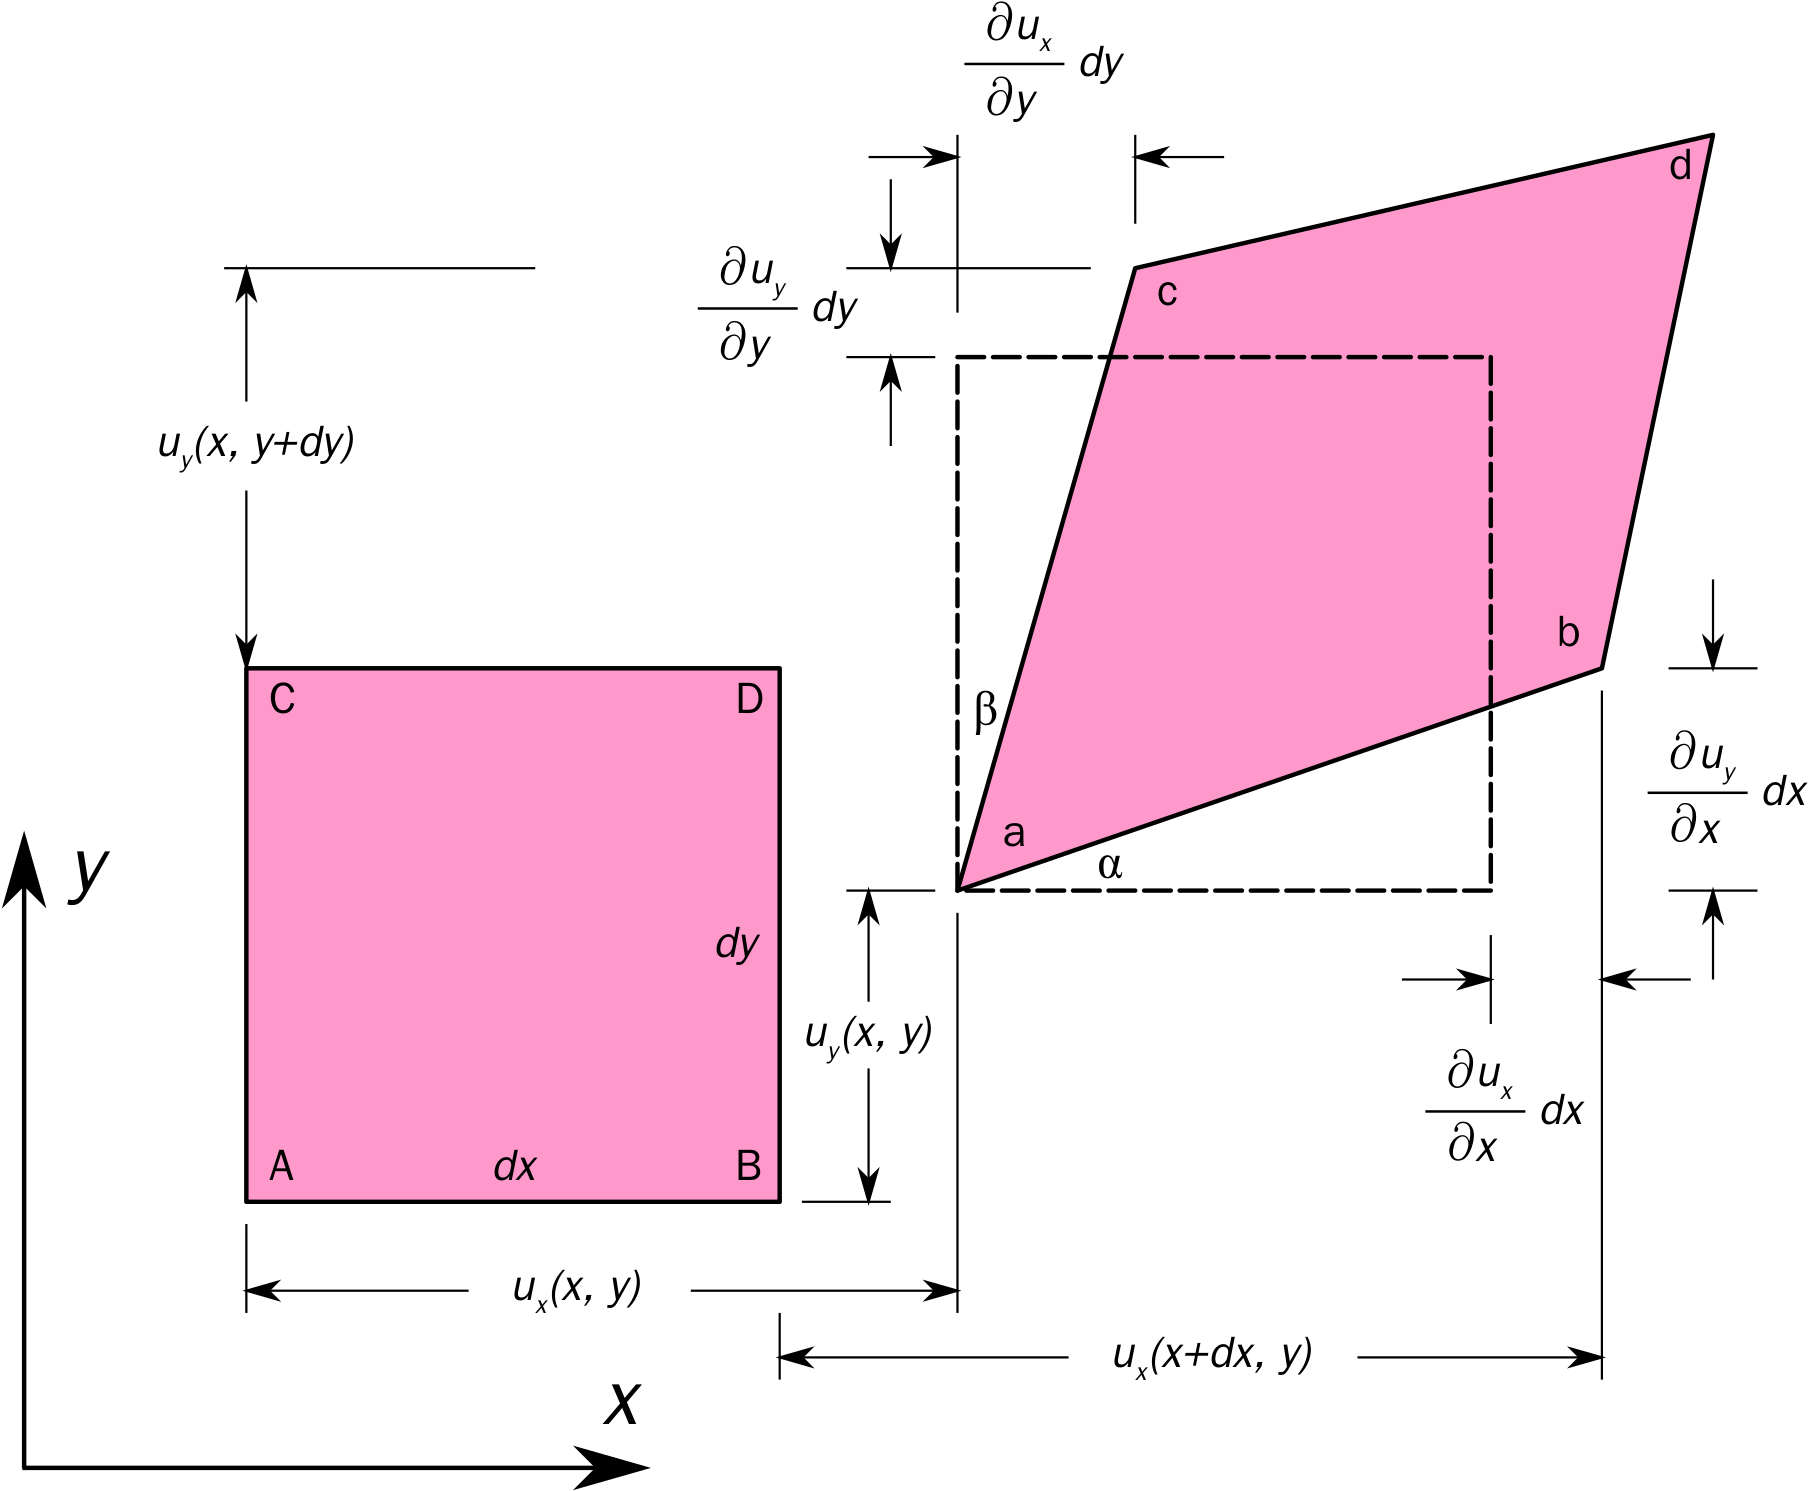
\includegraphics[width=100mm]{images/Strain_2D.png}}
  \caption{The Green-Lagrange strain tensor entries visualzied on a 2D $x,y$-plane. This also extends to 3 dimensions, but the visuals tend to get messy in 3 dimensions. Source: \url{https://commons.wikimedia.org/wiki/File:2D_geometric_strain.svg}}
\end{figure}


\subsection{Strain in a specified direction}
In some cases we are interested in finding the strain in a specific direction. This can be cases where we want to find strain along a specific fibre in a carbon-fibre composite for example. In this case we define a unit vector $\uvec{s}$ which lies parallel the fibre. The following relations apply to this unit vector:
\begin{gather}
  \d \vec{r} = \d r \uvec{s}\\
  ||\uvec{s}|| = 1
\end{gather}
We can then find the deformation in the direction of the unit vector $\uvec{s}$ using the dot product again:
\begin{equation}
  \epsilon =
  \begin{bmatrix}
    s_x &
    s_y &
    s_z
  \end{bmatrix}
  \begin{bmatrix}
    \epsilon_{xx} & \epsilon_{xy} & \epsilon_{xz} \\
    \epsilon_{yx} & \epsilon_{yy} & \epsilon_{yz} \\
    \epsilon_{zx} & \epsilon_{zy} & \epsilon_{zz} \\
  \end{bmatrix}
  \begin{bmatrix}
    s_x \\
    s_y \\
    s_z
  \end{bmatrix}
\end{equation}
Here $\epsilon$ represents the strain of the material along the fibre.
\end{document}